% Activate the following line by filling in the right side. If for example the name of the root file is Main.tex, write
% "...root = Main.tex" if the chapter file is in the same directory, and "...root = ../Main.tex" if the chapter is in a subdirectory.
 
%!TEX root =  ../Thesis.tex

\chapter[Background Estimation]{Background Estimation}

Once the background has been reduced as much as practical using the trigger and kinematic cuts,
a reliable estimate of the shape and size of the remaining background is critical to optimizing
the exclusion limits.  In particular, since the reconstructed mass peak of the $b$-jets is so
broad in signal, a mis-estimation of the background shape can lead to systematic errors that
could wash out any possible signal (or worse, be mistaken for a signal where there is none).  

At the same time, the backgrounds in this analysis are challenging to estimate, either in Monte
Carlo or using data-driven methods.  Therefore, much of the work of this analysis is dedicated
to validating the background estimation and providing uncertainties for especially the shape 
of the background.  

\section{Background Estimation Strategy}
\label{sec:background_strategy}
As QCD is the dominant background in this analysis, it is important to understand
what flavors of QCD jets compose the population of events that survive the cut
chain.  In order to do this, we apply the trigger and all cuts up to (but not including)
requiring a third $b$-tagged jet in the event.

 The signal and background are then split into 3 exclusive regions, defined as follows:
\begin{itemize}
    \item \textit{bbb}: one or more jets (in addition to the two triple-tagged jets) passing a tight (60\% working point)
 MV1 cut–-in effect, the full signal selection criteria
    \item \textit{bbloose}: events failing the bbb classification but which have one or more jets passing a loose (80\%
 working point) MV1 cut
    \item \textit{bbanti}: events that have no jets passing an 80\% MV1 cut-–effectively a veto on the presence of any
 $b$-tagged jets other than those firing the trigger
\end{itemize}



\section{Background Estimation Method Based on Exponential Background Model and Sideband Fitting}
The background consists almost exclusively of QCD with 2 or more real $b$-jets, which 
fortunately has a $m_{bb}$ spectrum that does not have any peaks or other difficult
structure above about 350 GeV.  Below that mass, the trigger turn-on curve becomes
a major feature of the spectrum.  Above that mass, there
is a smoothly falling distribution that we fit primarily with a decaying exponential.

In a few words, the background fit strategy proceeds in the following way:
\begin{itemize}
    \item Start with a mass point
    \item Apply a mass-point-specific rotation based on the the eigenvectors of 
    the signal MC, as calculated using $m_{bb}$, $p_{T}^1$ and $p_T^2$; call 
    the components of this rotated basis $m_{bb}'$, $p_T^{1'}$ and $p_T^{2'}$
    \item Apply cuts to $p_T^{1'}$ and $p_T^{2'}$, and use $m_{bb}^{'}$ as the final 
    discriminating variable 
%    \item Using the signal MC as a guide, select a window in $m_{bb}$ that encloses the
%signal peak, along with as much of the mass sideband (on either side) as possible
    \item Fit an exponential function to the $m_{bb}^{'}$ distribution, allowing each of the 
tag regions (\textit{bbb}, \textit{bbloose}, \textit{bbanti}) to float relative to each other
 as well as keeping the 3, 4, and 5+ jet categories separate
    \item As part of the limit-setting procedure, use the fit result for the 
    background along with signal shapes taken from MC to extract the 
signal cross section that can be excluded at a 95\% confidence level
    \item Repeat for the next mass point
\end{itemize}

Although we have signal MC with $m_A$ values as low as 250 GeV, this fit strategy only
begins to work above 400 GeV, because of the trigger turn-on curve.  The fit window
used is [340,900] GeV for all signal mass points.

While the analysis was in development, it was blinded to avoid bias.  This was done 
by removing \textit{bbb} events from the data, and replacing them with a sample of
events with the same normalization drawn from the \textit{bbanti} distribution
in data.  For the final search, the \textit{bbb} events were swapped back in.



%\section{Turn-On Curve Modeling}
%Although the lowest part of the $m_{bb}$ distribution (below 300 GeV) is not part of the search regime,
%because of the rapidly changing background, including it in the background model helps
%improve the overall fit by allowing for a slightly fewer events at moderately low
%$m_{bb}$ (between about 300 and 400 GeV) than an exponential alone would predict.
%The turn-on is fit with a logistic function of the form

%\begin{equation}
%f(m_{bb}) = N\frac{1}{1+e^{-c(m_{bb}+d)}}
%\end{equation}

%In this equation, N controls the overall normalization, $c$ governs the steepness
%of the turn-on curve, and $d$ is the horizontal offset.

%\textbf{once we confirm this (or something like it) as the final fit model,
%add a plot showing how this function changes with c/d and the composite
%model of exponential times logistic}


\section{Eigenvector Rotation}
\textbf{If Tim's eigen-analysis is validated and used, a description of that method goes here}

\begin{itemize}
    \item for high-mass points, we have trouble when FSR is bad (but it isn't always bad)
    \item FSR is worst when jets are low-pT--suggests a cut or categorization based
    on pT of the jets
    \item However, simple cut can sculpt background b/c of correlations btwn pT1, pT2, mbb,
    and it also reduces background to rates too low to model well
    \item use signal MC to identify eigenvectors based on pT1, pT2 and mbb, transform
    into this basis 
    \item Place cuts on pT1' and pt2'
    \item Use $mbb'$ as the discriminating variable, proceed to fit with exponential
    \item Impact on final sensitivity in the results section
\end{itemize}

Once the events have been categorized based on $b$-tag status and the number of jets in the
events, but before doing the final fit, we apply a change of variables based on the jet
$p_T$ values and $m_{bb}$ in each event and a kinematic cut.  Together these analysis 
steps effectively allow for a discriminating variable, which we call $m_{bb}'$, that
separates signal and background better than ordinary $m_{bb}$.  Once these steps have
been applied, the result is an analysis that is 15-50\% more sensitive
than if no transformation were applied.  This section will 
outline this procedure and its rationale.  

The motivation for this strategy has its origins in trying to control the effect of
FSR on the analysis sensitivity.  At high $m_A$, the jets from the Higgs (and also 
the associated $b$-quark) have large $p_T$, which they then tend to radiate away 
as FSR.  This causes the $m_{bb}$ peak to smear out and be more difficult to 
distinguish from background than in the lower-$m_A$ cases.  However, since FSR
occurs stochastically on an event-by-event basis, a subset of the signal events
will have little or no FSR and will reconstruct to $m_A$--if these events 
can be isolated from the others, they offer a chance to improve the sensitivity
via the improved mass resolution.  

A simple strategy might be to apply a cut to the $p_T$ of the leading and/or 
second jet in the event, and only accept events where the $p_T$ is above some
threshold optimized by comparing signal MC to \textit{bbanti} data.  
That would isolate events with poor mass resolution (i.e. lots of FSR) from
those with little FSR and better reconstruction properties.  However, since
there is a correlation between $p_T^1$, $p_T^2$ and $m_{bb}$, a cut like
this ends up sculpting the background as well.  In addition, the $p_T^1$ and
$p_T^2$ cut thresholds that looked best on signal MC are ``too good'' on 
background-dominated \textit{bbanti} events and there is no background
above a certain $m_{bb}$ value.  That makes modeling the background extremely 
difficult, and any fit difficult to validate.  






\section{Mathematical Modeling of Background Shape}
\subsection{Selection of Exponential Function}
say a few words on merits of exponential vs. power decay series,
bernstein polynomial, as well as 1-param vs. 2-param


\subsection{Background Shape and Spurious Signal}
\cite{spurious_signal}












\subsection{Non-QCD Backgrounds}
\label{sec:non_qcd_bkgs}

\subsubsection{All-Hadronic $t\bar{t}$ Background}
When $t\bar{t}$ decays all-hadronically, it can create events with several high-$p_T$
jets and 2 or more $b$-tagged jets (where the $b$-tags come from both real $b$-quarks
and from mistagged light flavor).  We anticipate that, because it has a production
cross section that is much smaller than QCD, $t\bar{t}$ will not be a major background.
We confirm this assumption in MC by using the all-hadronic $t\bar{t}$ sample summarized
in Table~\ref{tab:ttbar_params}.


We find that in MC, all-hadronic $t\bar{t}$ has an efficiency of 7.5\% after
the EF\_2j35\_loose\_j145\_j35\_a4tchad trigger, and approximately 2\% efficiency
in the offline cuts relative to the trigger.  Estimating the $t\bar{t}$ cross section
as 165 pb, and a 44\% branching ratio in the all-hadronic decay channel, this gives
a 0.11 pb $t\bar{t}$ cross section expected after the trigger and offline cuts.  In the
full 2012 dataset, this amounts to about 2400 events.  While
this is not a negligible cross section compared to the signal, it is more than an
order of magnitude smaller than the QCD background.

In addition to checking the magnitude of the $t\bar{t}$ background, we check the shape
for any shape differences in the $m_{bb}$ distribution depending on the tag status of the
third jet, and do not find any major discrepancies that point toward $t\bar{t}$ as a
potential peaking background in the signal region. The $m_{bb}$ distributions in the
bbb, bbloose and bbanti bins for the all-hadronic $t\bar{t}$ can be found in Figure
~\ref{fig:ttbar_mbb}.




\begin{figure}[hbt]
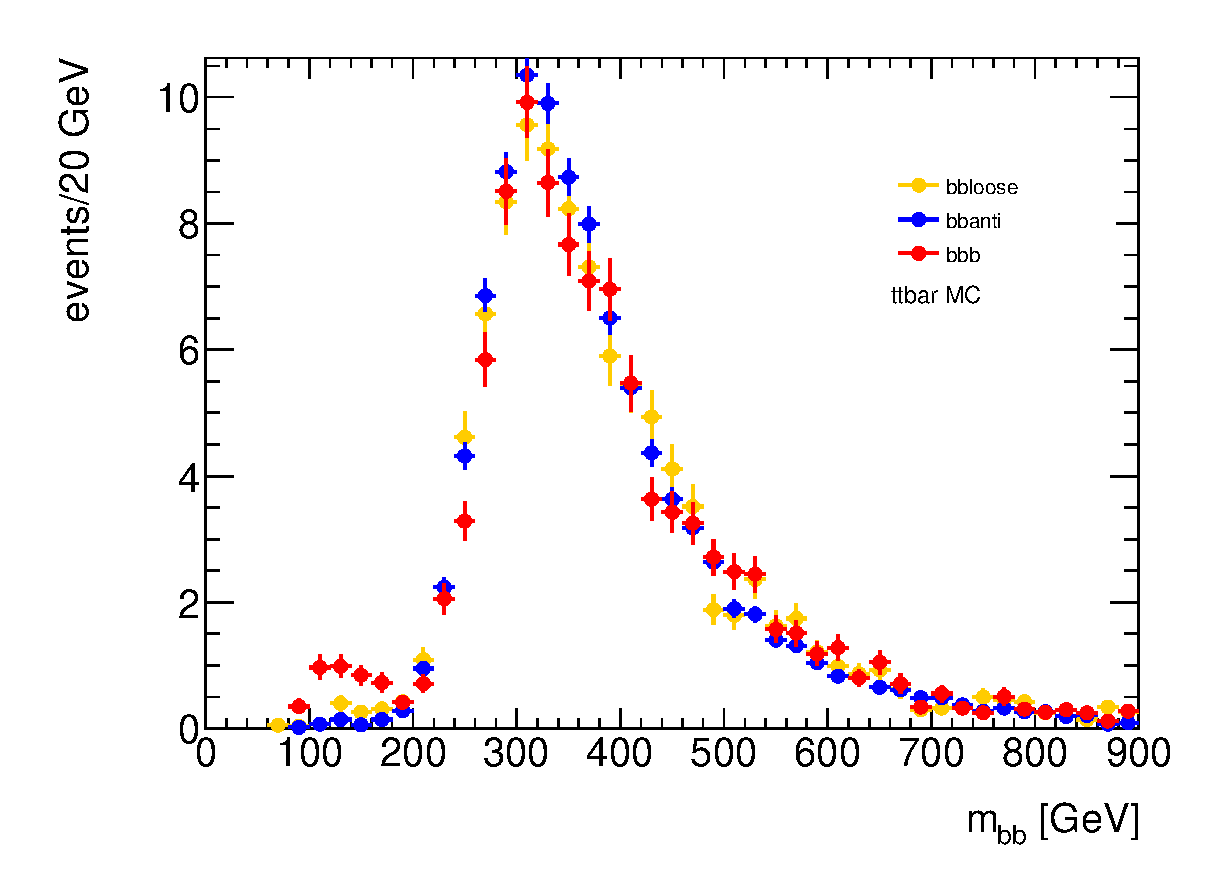
\includegraphics[width=0.45\linewidth]{BackgroundEstimation/images/mbb_compare_bbb_bbloose_bbanti_ttbar.eps}
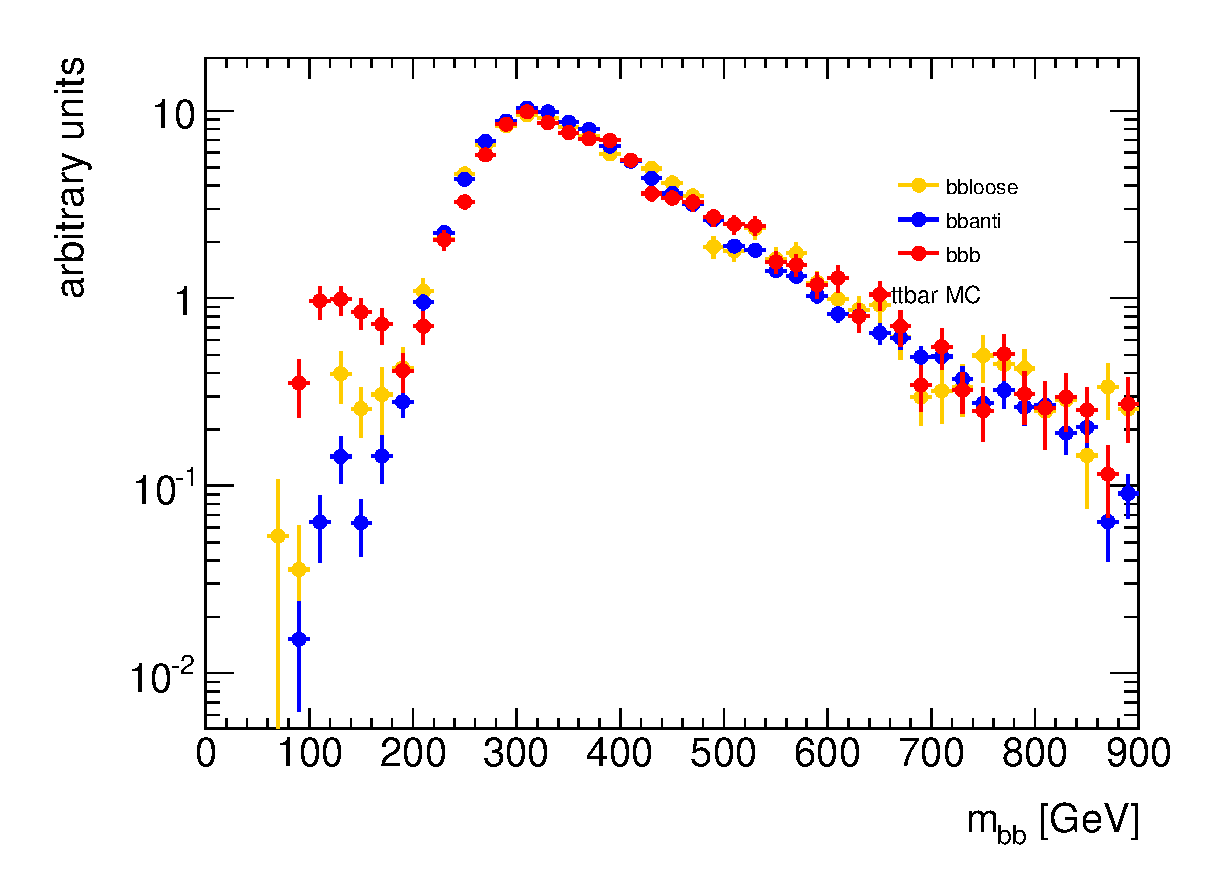
\includegraphics[width=0.45\linewidth]{BackgroundEstimation/images/mbb_compare_bbb_bbloose_bbanti_ttbar_logy.eps}
\caption{The $m_{bb}$ distributions for all-hadronic $t\bar{t}$ MC after the trigger and all offline cuts are applied (linear Y axis on the left, logarithmic scale on the right).  In addition to the overall cross-section, we also want to probe any shape differences that arise when the tag status changes on the third jet in the event.  No significant shape differences are seen.}
\label{fig:ttbar_mbb}
\end{figure}







%
%The background estimate is crucial to the analysis.  The QCD cross section at a hadron machine like the LHC is quite large; only a small subset of QCD events have 3 or more b-jets, but b-tagging does not have perfect performance and we expect a large contribution from QCD events in which one or more light or charm jets are b-tagged.
%
%The b-tagging in the trigger provides a handle for controlling the mistag background.  The L2, EF and offline MV1 b-tags are independent of each other, which is to say that (for example) the EF b-tagging decision on a given jet does not take into account whether the jet was tagged in L2, so we can improve the purity of our b-jet sample by requiring that the same jet pass L2, EF and MV1 tags.  




%The third jet in the event, however, will not be tagged by the trigger.  The jet will be tagged offline, but even after the offline tagging we expect there will be many events in which the third jet is not a b-jet, but is a mistagged light or charm jet.  The exact size of this background for light jets is given by equation \ref{eq:mistag}, and a similar equation can be written for charm jets.

%  \begin{equation}
%	N_{mistagged\ light\ jets} = N_{light\ jets} \times \epsilon_{light\ jet\ passing\ tag}
%\end{equation} \label{eq:mistag}

%The light mistag efficiency $\epsilon_{light\ jet\ passing\ tag}$ is computed and calibrated by the b-tagging performance group (see the b-tagging chapter for further details), so we need to compute the composition of light or charm jets in the original sample in order to estimate their contamination after b-tagging has been applied.  

%The QCD background is notoriously difficult to model in MC, and we find unacceptably low statistics in MC after our analysis cuts have been applied, so we use the data-driven matrix method to compute the QCD background composition as accurately as possible.  The matrix method makes use of the known efficiencies for tagging b, c and light jets, as well as information about how many jets pass a given b-tag, to arrive at 













